
\section{Ground cable routing}

Once the controller has been validated using the Stewart baseline, we can proceed to consider different ways to connect six ground cables to the platform (Figure \ref{fig:6ugvsConnections}) and the drone (Figure \ref{fig:3uavsConnections}). The same ground configuration hook-anchor can change the system's stability based on which hook is connected to which anchor point on the ground.
%% Why we choose the triangle for the UAVs configuration?
Therefore, we will start considering the drone attachment configuration as fixed to the triangular arrangement and vary only the routing of the six ground cables. This specific UAV configuration is chosen because it provides a symmetric distribution of the three drones around the payload. This approach allows one to isolate the influence of the ground cable routing and attribute differences in performance solely to the ground architecture. Finally, in Section \ref{sec:dronehook}, the impact of various UAV attachment geometries is examined independently.

%% How the code work, how a given cable routing has been found
Focusing on the ground cable routing, there are at most $6! = 720$ physically distinct valid ways to route the six ground cables. Scoring an architecture using only one arbitrarily chosen routing raise the question on how lucky the routing choice was and how good the architecture actually is. Therefore, implementing the selection strategy explained in Section \ref{sec:selection_strategy} is essential to make a guided choice and conclusions on the results.

\subsection{Ground screening}
\label{sec:ground_screening}
The pre-screening results are shown in Table \ref{tab:prescreening_feasibility} and Table \ref{tab:prescreening_index}, where ground cable routings were tested over 10 different poses.
Any routing that violates either WCC or IFC at any tested pose is removed, as it was explained deeply in Section \ref{sec:selection_strategy}.  For this reason, the WCC and IFC counts in Table \ref{tab:prescreening_feasibility} are per-routing failures, while the WFC count is not directly comparable, since it represents the total number of pose-level failures accumulated across all candidate routings. The WFC is the main cause of rejection, which means that many routings are still kinematically feasible, but they cannot produce the required wrench while keeping the cable tensions within the allowed range. The WCC failures are relatively few, indicating that rank deficiency is less common than tension infeasibility. IFC failures are only  caused by cable-cable interference, and not by exit-angle violations.

The quality of the selected routing is evaluated through four complementary metrics. The smallest singular value, $\sigma_{\min}$, measures the distance from singular configurations, while the conditioning index $\nu$ evaluates the isotropy of the wrench generation capability. Manipulability quantifies the overall size of the achievable wrench space, whereas $d_{\min}$ characterizes the minimum cable-to-cable clearance over all tested poses.

Table \ref{tab:prescreening_index} shows how no single architecture simultaneously maximizes every performance metric. The two-triangles-vertical-parallelepiped configuration provides the largest minimum singular value and the best conditioning index, indicating the greatest robustness against singular configurations. In contrast, the rectangle-opposite-2x3 architecture performs the highest manipulability, suggesting a larger overall wrench capability. Finally, the parallelepiped-int-2x3 layout provides the largest minimum cable clearance, reducing the likelihood of cable interference. These results highlight the trade-off between kinematic robustness, wrench capability, and geometric clearance.

\begin{table}[htbp]
\centering
\resizebox{\linewidth}{!}{
\begin{tabular}{lcccc}
\toprule
\textbf{Layout} & \textbf{WCC} & \textbf{WFC} & \textbf{IFC} & \\
\textbf{(Payload -- Ground)} & \textbf{Failures} & \textbf{Failures} & \textbf{Failures} & \textbf{Feasible} \\
\midrule
two-triangles -- vertical-parallelepiped    & 64 & 2538 & 507 & \checkmark \\
rectangle-opposite -- 2X3                    & 72 & 146  & 94  & \checkmark \\
parallelepiped-int -- 2X3                   & 52 & 340  & 102 & \checkmark \\
parallelepiped-ext -- horizzontal-parallelepiped & 24 & 630 & 116 & \checkmark \\
central-trapezoid -- horizzontal-parallelepiped  & 16 & 1186 & 255 & \checkmark \\
\bottomrule
\end{tabular}
}
\caption{Pre-screening feasibility of cable-routing architectures}
\label{tab:prescreening_feasibility}
\end{table}

\begin{table}[htbp]
\centering
\begin{threeparttable}

\begin{tabular}{lcccc}
\toprule
\textbf{Layout (Payload -- Ground)} & $\sigma_{\min}$ \tnote{a} & $\nu$ \tnote{b} & $w$ \tnote{c}& $d_{\min}$ \tnote{d}  \\
\midrule
two-triangles -- vertical-parallelepiped    & 0.1911 & 0.0797 & 0.0450       & 0.0638 \\
rectangle-opposite -- 2X3                    & 0.1875 & 0.0786 & 0.0957      & 0.2027 \\
parallelepiped-int -- 2X3                   & 0.1892 & 0.0784 & 0.0344       & 0.3213 \\
parallelepiped-ext -- horizzontal-parallelepiped & 0.1825 & 0.0750 & 0.0302  & 0.1921 \\
central-trapezoid -- horizzontal-parallelepiped  & 0.1676 & 0.0696 & 0.0290  & 0.1452 \\
\bottomrule
\end{tabular}
\caption{Best routing quality across feasible architectures}
\label{tab:prescreening_index}

\begin{tablenotes}
\footnotesize
\item[a] $\sigma_{\min}$ = smallest singular value of the payload Jacobian.
\item[b] $\nu$ = conditioning index (Eq. \ref{eq:conditioning_index})
\item[c] $w$ = manipulability (Eq. \ref{eq:manipulability})
\item[d] $d_{\min}$ = minimum cable-to-cable clearance of the selected routing over all tested poses.
\end{tablenotes}
\end{threeparttable}
\end{table}


\todo[inline]{Talk about triangle-triangle combination why it does not pass the pre-screening?}

Notice something very odd. It never even reached WCC/WFC/IFC failures. This suggests the algorithm never found a routing to evaluate, or the architecture was rejected before the screening loop. That is not something you can conclude from the tables.

I would first verify the code. If it is indeed skipped because: payload layout equals ground layout, or there are only six identical permutations, then discuss that.

% This is the result triangle-triangle
% pay_layout	gnd_layout	n_routings_checked	n_poses_checked	feasible	n_wcc_fail	n_wfc_fail	n_ifc_fail	n_ifc_fail_cable_cable	n_ifc_fail_exit_angle	wfc_fail_residual_min	wfc_fail_residual_median	wfc_fail_residual_max	wfc_fail_residual_force_median	wfc_fail_residual_moment_median	wfc_fail_residual_force_lateral_median	wfc_fail_residual_force_vertical_median	n_wfc_verify_attempted	n_wfc_verify_rescued	conditioning_index	manipulability	sigma_min	sigma_max	rank_ok	wfc_ok	max_wfc_residual	max_wfc_residual_force	max_wfc_residual_moment	ifc_ok	min_cable_cable_dist	min_exit_angle_margin	wfc_rescued_by_reposition	best_routing
% triangle	triangle	6	10	False	0	0	0	0	0								0	0	



\subsection{Simulation run}
%% How and why the results before simulation and after simulation differ?
The theoretical indices evaluate the geometric and static properties of a cable routing. They define configurations close to kinematic or wrench singularities, and they classify architectures based on their ability to generate payload wrenches. However, they cannot predict the transient response of the closed-loop system. Dynamic effects such as payload inertia and load redistribution are only captured by simulation. Therefore, while poor theoretical indices almost always indicate poor dynamic performance, the opposite is not necessarily true: a routing with good static indices may still have oscillations or bad tracking.

For each configuration derived in the previous step, a simulation is run over 60 different poses (shown in Figure \ref{fig:test_poses}), and conclusions are drawn. Additionally, extra simulations have been run to test specific ground cable routing and see if they lead us to further conclusions. Table \ref{tab:architecture_ranking} summarizes the results of the dynamic simulations for the candidate architectures selected during the pre-screening. The objective is to evaluate whether the theoretical metrics introduced previously are consistent with the observed closed-loop behavior. In particular, the simulations assess pose reachability, cable rubbing and numerical stability over the set of 60 testing poses. Each indicator is ranked from 1 to 5, where lower values correspond to better overall performance.


\begin{figure}
    \centering
    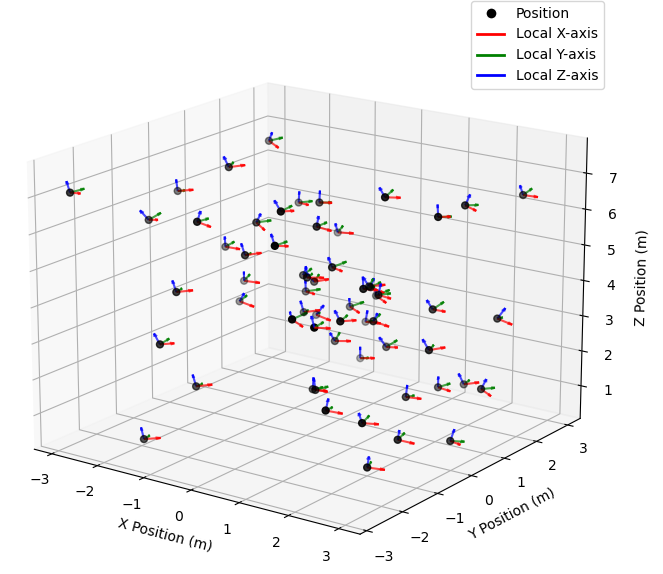
\includegraphics[width=0.65\linewidth]{images/testing_poses.png}
    \caption{Testing poses}
    \label{fig:test_poses}
\end{figure}


\begin{table}[htbp]
\centering
\begin{threeparttable}
\resizebox{\linewidth}{!}{
\begin{tabular}{l c c c c c c}
\toprule
\textbf{Architecture} & $\nu$ & $w$ & $N$ & \textbf{Pose Reach} & \textbf{Cable Rub} & \textbf{Instab.} \\
\midrule
rectangle-opposite-2x3 & 0.1246 (1) & 1.0459 (1) & 8.9142 (1) & 0.5833 (5) & 0.9333 (6) & 0.0500 (2) \\
parallel-int-2x3 & 0.0997 (4) & 0.4536 (4) & 6.7857 (2) & 0.7500 (1) & 0.4667 (3) & 0.0500 (2) \\
two-triangles-vertical-parallel & 0.1107 (3) & 0.4907 (3) & 5.9310 (3) & 0.6667 (3) & 0.9167 (5) & 0.0667 (5) \\
parallel-ext-horiz-parallel & 0.1210 (2) & 0.7770 (2) & 5.8649 (4) & 0.5333 (6) & 0.4500 (2) & 0.0500 (2) \\
acts\_stewart & 0.0533 (6) & 0.1054 (6) & 5.5706 (5) & 0.6500 (4) & 0.3167 (1) & 0.0833 (6) \\
central-trapezoid-horiz-parallel & 0.0803 (5) & 0.2099 (5) & 4.8839 (6) & 0.7333 (2) & 0.6333 (4) & 0.0333 (1) \\
\bottomrule
\end{tabular}
}
\caption{Static and dynamic performance indices for the six candidate architectures, with rank (1 = best, 6 = worst) shown in parentheses.}
\label{tab:architecture_ranking}
\begin{tablenotes}
\footnotesize
\item $\nu$ = conditioning index; $w$ = manipulability; $N$ = composite score; 
\item Pose Reach = fraction of trials reaching the target pose; 
\item Cable Rub = fraction of trials with cable rubbing; 
\item Instab. = \texttt{simulation\_unstable} rate. 
\end{tablenotes}
\end{threeparttable}
\end{table}


\todo[inline]{What does the table tells us about?}
For instance, the rectangle-opposite-2x3 architecture achieves the highest conditioning index and manipulability, yet exhibits the lowest pose reachability and the highest cable rubbing rate. Conversely, the parallelepiped-int-2x3 and central-trapezoid-horizontal-parallelepiped architectures provide better dynamic performance despite lower theoretical rankings. These results indicate that geometric quality alone is insufficient to characterize the overall behavior of the system, as dynamic effects such as payload inertia, cable force redistribution, and controller interaction become dominant during motion. The ACTS Stewart platform serves as a baseline reference, illustrating how the hybrid cable-driven architectures compare against the conventional parallel manipulator. Overall, the simulations validate the role of the pre-screening in eliminating infeasible routings while demonstrating the necessity of dynamic simulation for selecting the most suitable architecture.

\todo[inline]{How the results before simulation and after simulation differ?}

The dynamic simulations reveal that the theoretical performance indices alone do not fully predict the closed-loop behaviour of the system. The rectangle-opposite-2x3 architecture, which achieves the highest conditioning index and manipulability, exhibits the lowest pose reachability and one of the highest cable rubbing rates. Conversely, the parallelepiped-int-2x3 architecture, despite a lower conditioning index and manipulability, achieves the highest pose reachability while maintaining moderate cable interference. Similarly, the central-trapezoid-horizontal-parallelepiped architecture, which ranks lowest in the theoretical indices among the cable-driven configurations, presents the lowest instability rate. These observations indicate that the static metrics are effective for identifying geometrically favourable routings and avoiding singular configurations, but they do not account for dynamic effects such as payload inertia, force redistribution between cables, and the interaction with the controller.

Supplementary simulations have been run on configurations realized manually, rather than selected through a systematic search.

\todo[inline]{Does this give us additional results?}

The supplementary manually designed configurations further demonstrate that the cable routing itself has a significant influence on the dynamic behavior, even when the underlying payload and ground geometries remain unchanged. Architectures sharing the same layouts but employing different cable assignments exhibit noticeable differences in pose reachability, cable rubbing and instability.

Overall, the manually selected routings do not consistently outperform those obtained through the systematic screening procedure. This suggests that manually identifying a suitable routing based solely on geometric intuition is difficult, whereas the proposed screening strategy provides a more reliable and reproducible means of selecting high-quality candidate routings for subsequent dynamic evaluation.

\begin{table}[htbp]
\centering
\begin{threeparttable}
\resizebox{\linewidth}{!}{
\begin{tabular}{lcccccc}
\toprule
\textbf{Architecture} & $\nu$ & $w$ & $N$ & \textbf{Pose Reach} & \textbf{Cable Rub} & \textbf{Instab.} \\
\midrule
rect-same--rect-opposite & 0.1077 (2) & 9.1356 (1) & 9.1356 (1) & 0.6167 (5) & 1.0000 (4) & 0.2500 (3)\\
2X3--rect-same & 0.1226 (1) & 8.5115 (2) & 8.5115 (2) & 0.7000 (3) & 1.0000 (4) & 0.4833 (5) \\
horiz-parall.--horiz-parall.-3 & 0.0647 (3) & 6.6252 (3) & 6.6252 (3) & 0.7833 (1) & 0.4000 (1) & 0.0667 (1) \\
horiz-parall.--horiz-parall. & 0.0645 (4) & 6.5651 (4) & 6.5651 (4) & 0.7167 (2) & 1.0000 (4) & 0.2500 (3)\\
rect-opposite--2X3-2 & 0.1126 (5) & 6.4080 (5) & 6.4080 (5) & 0.5667 (4) & 1.0000 (4) & 0.1667 (2) \\
\bottomrule
\end{tabular}
}
\caption{Top five manual architectures}
\label{tab:architecture_ranking_manual}

\end{threeparttable}
\end{table}

\subsection{Analysis of Specific configurations}
\subsubsection{Degenerative ground configurations - Line and Diagonal}
\label{sec:degenerativeConfigurationa}
The exhaustive screening consistently rejects the line and diagonal ground-routing configurations. This result is expected, as in these layouts several cable directions become nearly coplanar or aligned, resulting in cable arrangements that are close to kinematic singularities. Consequently, the cable system can no longer generate a full six-dimensional wrench space. This result could have also been explained geometrically. In the line configuration, cable attachments lie along a single axis, which limits the system's ability to generate forces and torques in directions perpendicular to that line. Similarly, the diagonal configuration introduces a strong directional bias along the axis on which the cable attachments are positioned.

Simulation results using hand-crafted configurations confirm this conclusion: line-based and diagonal-based ground cable layouts never rank among the highest-performing architectures in terms of composite score. The drop in performance becomes particularly pronounced when both the payload and the ground attachments are arranged in a one-dimensional configuration. In such cases, the desired pose is achieved less than half the time, like in the line-line-triangle configuration that succeeds only 40\% of the time. Success rates nearly double when at least one attachment expands into two dimensions, as seen in line-pentagon-triangle (56.67\%) or line-hexagon-triangle (76.67\%).

\subsubsection{Configuration two-triangles--vertical-parallelepiped--triangle}

two-triangles-vertical-parallelepiped has the largest $\sigma_{min}$, it also has the largest conditioning index, but it has lower manipulability than rectangle-opposite. This is nice because it illustrates that: manipulability measures the overall volume of the wrench ellipsoid, whereas $\sigma_{min}$ measures the worst-case direction. So an architecture can have: slightly smaller manipulability, but a larger $\sigma_{min}$, meaning it is more isotropic and farther from singularity, even if its total wrench capability is not maximal.

The simulation results further show that neither property alone determines the dynamic performance. Although the two-triangles-vertical-parallelepiped architecture provides the largest $\sigma_{\min}$, indicating the greatest robustness against singular configurations, it does not achieve the best closed-loop performance. Likewise, the rectangle-opposite-2x3 architecture, which maximizes manipulability, performs poorly in terms of pose reachability. Therefore, $\sigma_{\min}$ and manipulability should be interpreted as complementary geometric indicators rather than direct predictors of dynamic behavior.


\todo[inline]{Other combinations that give interesting results?}
Overall, the simulation results indicate that no single architecture simultaneously optimizes every performance metric. The rectangle-opposite-2x3 architecture maximizes the theoretical indices, whereas the central-trapezoid-horizontal-parallelepiped architecture provides the highest numerical stability. The parallelepiped-int-2x3 architecture, however, offers the best overall compromise by combining the highest pose reachability with low instability and acceptable cable rubbing. Relative to the ACTS Stewart baseline, it demonstrates that the proposed cable-driven architecture can achieve comparable closed-loop performance while satisfying the additional routing constraints inherent to the hybrid system.